\documentclass[aspectratio=169]{beamer}

% =====================================================
% THEME
% =====================================================
\usetheme{Madrid}
\usecolortheme{seahorse}

% =====================================================
% PACKAGES
% =====================================================
\usepackage[T1]{fontenc}
\usepackage{lmodern}
\usepackage{listings}
\usepackage{xcolor}
\usepackage{tikz}
\usepackage{booktabs}
\usepackage{array}
\usepackage{amsmath}

\usetikzlibrary{
    arrows.meta,
    positioning,
    shapes.geometric
}

% =====================================================
% COLORS
% =====================================================
\definecolor{codebg}{RGB}{248,248,248}
\definecolor{keyword}{RGB}{0,80,150}
\definecolor{comment}{RGB}{80,110,80}
\definecolor{stringcolor}{RGB}{170,40,40}

% =====================================================
% CODE STYLE
% =====================================================
\lstdefinestyle{cstyle}{
    language=C,
    basicstyle=\ttfamily\scriptsize,
    keywordstyle=\color{keyword}\bfseries,
    commentstyle=\color{comment},
    stringstyle=\color{stringcolor},
    backgroundcolor=\color{codebg},
    frame=single,
    rulecolor=\color{gray!40},
    breaklines=true,
    showstringspaces=false,
    tabsize=4,
    numbers=left,
    numberstyle=\tiny\color{gray},
    numbersep=7pt,
    xleftmargin=0.3cm,
    framexleftmargin=0.2cm
}

% =====================================================
% PRESENTATION DETAILS
% =====================================================
\title[OS Lab -- Week 5]{Implementation of Pipe}

\subtitle{Operating Systems Laboratory -- Week 5}

\author{Dr. Siddhant Thapliyal}

\institute{
Department of Computer Science and Engineering\\
Graphic Era Deemed to be University
}

\date{\today}

% =====================================================
% DOCUMENT
% =====================================================
\begin{document}

% =====================================================
% SLIDE 1
% =====================================================
\begin{frame}
    \titlepage
\end{frame}

% =====================================================
% SLIDE 2
% =====================================================
% \begin{frame}{Aim}

% \begin{block}{Aim of the Experiment}
% To implement \textbf{Inter-Process Communication (IPC)}
% between related processes using an unnamed pipe.
% \end{block}

% \vspace{0.4cm}

% By the end of this laboratory session, students will be able to:

% \begin{itemize}
%     \item Explain the need for Inter-Process Communication.
%     \item Understand how an unnamed pipe works.
%     \item Explain the purpose of \texttt{pipe()}.
%     \item Differentiate between \texttt{fd[0]} and \texttt{fd[1]}.
%     \item Use \texttt{read()} and \texttt{write()} with pipes.
%     \item Use \texttt{fork()} and \texttt{pipe()} together.
%     \item Close unused pipe ends correctly.
%     \item Implement communication between parent and child processes.
% \end{itemize}

% \end{frame}

% =====================================================
% SLIDE 3
% =====================================================
\begin{frame}{What is Inter-Process Communication?}

\begin{block}{Definition}
Inter-Process Communication (IPC) refers to mechanisms provided by the
operating system that allow processes to exchange data and coordinate
their activities.
\end{block}

\begin{itemize}
    \item Processes normally have separate address spaces.
    \item One process cannot directly access the local variables of another.
    \item IPC provides controlled mechanisms for communication.
\end{itemize}

\begin{alertblock}{Why IPC?}
Processes often need to cooperate, exchange results, share data,
or synchronize their execution.
\end{alertblock}

\end{frame}

% =====================================================
% SLIDE 4
% =====================================================
\begin{frame}{Common IPC Mechanisms in Linux}

Common IPC mechanisms include:

\begin{enumerate}
    \item Pipe
    \item FIFO / Named Pipe
    \item Message Queue
    \item Shared Memory
    \item Semaphore
    \item Signals
    \item Sockets
\end{enumerate}

\vspace{0.3cm}

\begin{block}{Week 5 Focus}
In this session, we focus on the simplest classical IPC mechanism:
\textbf{Unnamed Pipe}.
\end{block}

\end{frame}

% =====================================================
% SLIDE 5
% =====================================================
\begin{frame}{What is a Pipe?}

\begin{block}{Definition}
A pipe is an IPC mechanism that provides a
\textbf{unidirectional data channel} between processes.
\end{block}

\begin{itemize}
    \item Data written at one end can be read from the other end.
    \item Pipes are commonly used between related processes.
    \item Parent and child can communicate after \texttt{fork()}.
    \item A pipe behaves like a byte stream.
    \item Data normally flows in one direction.
\end{itemize}

\begin{center}
\Large
Writer $\longrightarrow$ Pipe $\longrightarrow$ Reader
\end{center}

\end{frame}

% =====================================================
% SLIDE 6
% =====================================================
\begin{frame}{The \texttt{pipe()} System Call}

\begin{block}{Prototype}
\centering
\texttt{int pipe(int fd[2]);}
\end{block}

Required header:

\begin{center}
\texttt{\#include <unistd.h>}
\end{center}

\vspace{0.3cm}

The call:

\begin{center}
\texttt{pipe(fd);}
\end{center}

creates two file descriptors.

\begin{center}
\begin{tabular}{|c|c|}
\hline
\textbf{Descriptor} & \textbf{Purpose} \\
\hline
\texttt{fd[0]} & Read end of the pipe \\
\hline
\texttt{fd[1]} & Write end of the pipe \\
\hline
\end{tabular}
\end{center}

\end{frame}

% =====================================================
% SLIDE 7
% =====================================================
\begin{frame}{Visualizing a Pipe}

\begin{center}

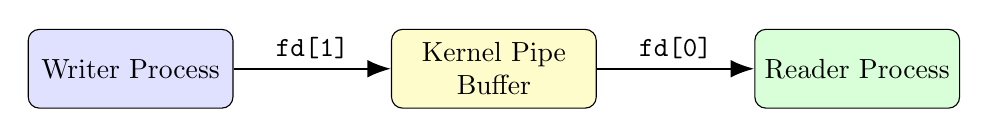
\begin{tikzpicture}[
node distance=1.5cm,
box/.style={
draw,
rounded corners,
minimum width=2.6cm,
minimum height=1cm,
align=center
}
]

\node[box, fill=blue!12] (writer)
{Writer Process};

\node[box, fill=yellow!20,
right=2cm of writer] (pipe)
{Kernel Pipe\\Buffer};

\node[box, fill=green!15,
right=2cm of pipe] (reader)
{Reader Process};

\draw[-{Latex[length=3mm]}, thick]
(writer) -- node[above]{\texttt{fd[1]}} (pipe);

\draw[-{Latex[length=3mm]}, thick]
(pipe) -- node[above]{\texttt{fd[0]}} (reader);

\end{tikzpicture}

\end{center}

\vspace{0.4cm}

\begin{alertblock}{Remember}
\texttt{fd[1]} is used for writing,
while \texttt{fd[0]} is used for reading.
\end{alertblock}

\end{frame}

% =====================================================
% SLIDE 8
% =====================================================
\begin{frame}{Return Value of \texttt{pipe()}}

The \texttt{pipe()} system call returns:

\begin{center}
\begin{tabular}{|c|p{7cm}|}
\hline
\textbf{Return Value} & \textbf{Meaning} \\
\hline

0 &
Pipe created successfully.
\\
\hline

-1 &
Pipe creation failed and \texttt{errno} is set.
\\
\hline

\end{tabular}
\end{center}

\vspace{0.3cm}

Good programming practice:

\begin{center}
\texttt{if (pipe(fd) == -1)}\\
\texttt{\{}\\
\texttt{\quad perror("pipe");}\\
\texttt{\quad return 1;}\\
\texttt{\}}
\end{center}

\end{frame}

% =====================================================
% SLIDE 9
% =====================================================
\begin{frame}{Why Do We Use \texttt{fork()} with a Pipe?}

A pipe created before \texttt{fork()} is inherited by the child.

Therefore:

\begin{enumerate}
    \item Parent creates the pipe.
    \item Parent calls \texttt{fork()}.
    \item Child inherits both pipe descriptors.
    \item Parent and child can use the descriptors to communicate.
\end{enumerate}

\begin{alertblock}{Important Order}
Normally:
\[
\boxed{
\texttt{pipe()}
\rightarrow
\texttt{fork()}
\rightarrow
\texttt{read()/write()}
}
\]
\end{alertblock}

\end{frame}

% =====================================================
% SLIDE 10
% =====================================================
\begin{frame}{Pipe Before and After \texttt{fork()}}

Before \texttt{fork()}:

\begin{center}
Parent Process $\longrightarrow$ \texttt{fd[0], fd[1]}
\end{center}

After \texttt{fork()}:

\begin{center}
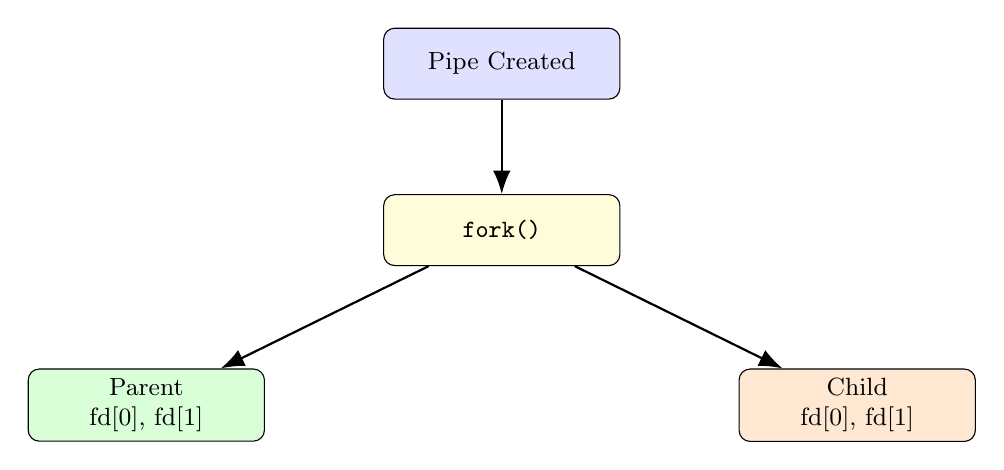
\begin{tikzpicture}[
node distance=1.4cm,
box/.style={
draw,
rounded corners,
minimum width=3cm,
minimum height=0.9cm,
align=center,
font=\small
}
]

\node[box, fill=blue!12] (pipe)
{Pipe Created};

\node[box, fill=yellow!15,
below=1.2cm of pipe] (fork)
{\texttt{fork()}};

\node[box, fill=green!15,
below left=1.3cm and 1.5cm of fork] (parent)
{Parent\\fd[0], fd[1]};

\node[box, fill=orange!18,
below right=1.3cm and 1.5cm of fork] (child)
{Child\\fd[0], fd[1]};

\draw[-{Latex[length=3mm]}, thick]
(pipe) -- (fork);

\draw[-{Latex[length=3mm]}, thick]
(fork) -- (parent);

\draw[-{Latex[length=3mm]}, thick]
(fork) -- (child);

\end{tikzpicture}
\end{center}

\end{frame}

% =====================================================
% SLIDE 11
% =====================================================
\begin{frame}{Important Question}

After \texttt{fork()}, both processes possess:

\begin{center}
\texttt{fd[0]} and \texttt{fd[1]}
\end{center}

But suppose:

\begin{itemize}
    \item Child should only write.
    \item Parent should only read.
\end{itemize}

Then:

\begin{center}
Child should close \texttt{fd[0]}.
\end{center}

and

\begin{center}
Parent should close \texttt{fd[1]}.
\end{center}

\begin{alertblock}{Good Practice}
Always close the unused end of the pipe.
\end{alertblock}

\end{frame}

% =====================================================
% SLIDE 12
% =====================================================
\begin{frame}{Correct Descriptor Usage}

Suppose communication is:

\[
\text{Child} \longrightarrow \text{Parent}
\]

Then:

\begin{center}
\begin{tabular}{|c|c|c|}
\hline
\textbf{Process} & \textbf{Close} & \textbf{Use} \\
\hline

Child &
\texttt{fd[0]} &
\texttt{fd[1]} for writing
\\
\hline

Parent &
\texttt{fd[1]} &
\texttt{fd[0]} for reading
\\
\hline

\end{tabular}
\end{center}

\vspace{0.4cm}

\[
\boxed{
Child
\xrightarrow{\texttt{write(fd[1],...)}}
Pipe
\xrightarrow{\texttt{read(fd[0],...)}}
Parent
}
\]

\end{frame}

% =====================================================
% SLIDE 13
% =====================================================
\begin{frame}{The \texttt{write()} System Call}

\begin{block}{Prototype}
\centering
\texttt{ssize\_t write(int fd, const void *buf, size\_t count);}
\end{block}

\begin{itemize}
    \item Writes data to a file descriptor.
    \item For a pipe, use the write end:
    \begin{center}
    \texttt{fd[1]}
    \end{center}
    \item \texttt{buf} contains the data.
    \item \texttt{count} specifies how many bytes to write.
    \item Return value gives the number of bytes written.
\end{itemize}

Example:

\begin{center}
\texttt{write(fd[1], message, strlen(message) + 1);}
\end{center}

\end{frame}

% =====================================================
% SLIDE 14
% =====================================================
\begin{frame}{The \texttt{read()} System Call}

\begin{block}{Prototype}
\centering
\texttt{ssize\_t read(int fd, void *buf, size\_t count);}
\end{block}

\begin{itemize}
    \item Reads data from a file descriptor.
    \item For a pipe, use:
    \begin{center}
    \texttt{fd[0]}
    \end{center}
    \item The received data is stored in a buffer.
    \item Return value gives the number of bytes read.
\end{itemize}

Example:

\begin{center}
\texttt{read(fd[0], buffer, sizeof(buffer));}
\end{center}

\end{frame}

% =====================================================
% SLIDE 15
% =====================================================
\begin{frame}{The \texttt{close()} System Call}

\begin{block}{Prototype}
\centering
\texttt{int close(int fd);}
\end{block}

Used to close a file descriptor that is no longer required.

Examples:

\begin{center}
\texttt{close(fd[0]);}
\end{center}

or

\begin{center}
\texttt{close(fd[1]);}
\end{center}

\begin{alertblock}{Why Close Unused Ends?}
Leaving unnecessary descriptors open can cause resource leaks and may also
prevent a reader from detecting end-of-file correctly.
\end{alertblock}

\end{frame}

% =====================================================
% SLIDE 16
% =====================================================
\begin{frame}[fragile]{Basic Pipe Program}

\begin{lstlisting}[style=cstyle]
#include <stdio.h>
#include <stdlib.h>
#include <string.h>
#include <unistd.h>
#include <sys/wait.h>

int main(void)
{
    int fd[2];
    pid_t pid;

    char message[] = "Hello from Child";
    char buffer[100];

    if (pipe(fd) == -1)
    {
        perror("pipe");
        return EXIT_FAILURE;
    }

    pid = fork();
\end{lstlisting}

\end{frame}

% =====================================================
% SLIDE 17
% =====================================================
\begin{frame}[fragile]{Basic Pipe Program -- Continued}

\begin{lstlisting}[style=cstyle]
    if (pid < 0)
    {
        perror("fork");
        return EXIT_FAILURE;
    }
    else if (pid == 0)
    {
        close(fd[0]);

        write(fd[1],
              message,
              strlen(message) + 1);

        close(fd[1]);
    }
    else
    {
        close(fd[1]);

        read(fd[0],
             buffer,
             sizeof(buffer));

        printf("Parent received: %s\n",
               buffer);

        close(fd[0]);

        wait(NULL);
    }

    return EXIT_SUCCESS;
}
\end{lstlisting}

\end{frame}

% =====================================================
% SLIDE 18
% =====================================================
\begin{frame}{Execution Flow}

\begin{enumerate}

    \item \texttt{pipe(fd)} creates the communication channel.

    \item \texttt{fork()} creates the child process.

    \item Child closes the read end.

    \item Child writes data using:
    \begin{center}
    \texttt{write(fd[1], ...)}
    \end{center}

    \item Parent closes the write end.

    \item Parent reads using:
    \begin{center}
    \texttt{read(fd[0], ...)}
    \end{center}

    \item Parent displays the received message.

\end{enumerate}

\end{frame}

% =====================================================
% SLIDE 19
% =====================================================
\begin{frame}{Expected Output}

For the previous program:

\begin{block}{Output}
\texttt{Parent received: Hello from Child}
\end{block}

\vspace{0.5cm}

Data flow:

\[
\boxed{
Child
\rightarrow
fd[1]
\rightarrow
Kernel Pipe
\rightarrow
fd[0]
\rightarrow
Parent
}
\]

\end{frame}

% =====================================================
% SLIDE 20
% =====================================================
\begin{frame}[fragile]{Lab Manual Program}

\begin{lstlisting}[style=cstyle]
#include <stdio.h>
#include <stdlib.h>
#include <string.h>
#include <unistd.h>
#include <sys/wait.h>

int main(void)
{
    int fd[2];
    pid_t pid;

    char message[100];
    char buffer[100];

    if (pipe(fd) == -1)
    {
        perror("pipe");
        return EXIT_FAILURE;
    }

    pid = fork();
\end{lstlisting}

\end{frame}

% =====================================================
% SLIDE 21
% =====================================================
\begin{frame}[fragile]{Lab Manual Program -- Continued}

\begin{lstlisting}[style=cstyle]
    if (pid == 0)
    {
        close(fd[0]);

        printf("Enter a string: ");
        fgets(message,
              sizeof(message),
              stdin);

        write(fd[1],
              message,
              strlen(message) + 1);

        close(fd[1]);

        exit(EXIT_SUCCESS);
    }
    else
    {
        close(fd[1]);

        read(fd[0],
             buffer,
             sizeof(buffer));

        printf("Parent received: %s",
               buffer);

        close(fd[0]);

        wait(NULL);
    }

    return EXIT_SUCCESS;
}
\end{lstlisting}

\end{frame}

% =====================================================
% SLIDE 22
% =====================================================
\begin{frame}{Sample Output}

\begin{block}{Execution}
\texttt{Enter a string: Graphic Era}\\[0.2cm]

\texttt{Parent received: Graphic Era}
\end{block}

\vspace{0.5cm}

\begin{block}{Observation}
The child obtains input from the user and sends it through the pipe.
The parent receives and displays the data.
\end{block}

\end{frame}

% =====================================================
% SLIDE 23
% =====================================================
\begin{frame}{Where is Pipe Data Stored?}

Pipe data is managed by the operating-system kernel.

\begin{center}

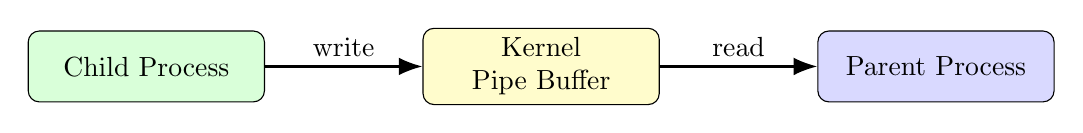
\begin{tikzpicture}[
node distance=1.5cm,
box/.style={
draw,
rounded corners,
minimum width=3cm,
minimum height=0.9cm,
align=center
}
]

\node[box, fill=green!15] (child)
{Child Process};

\node[box, fill=yellow!20,
right=2cm of child] (kernel)
{Kernel\\Pipe Buffer};

\node[box, fill=blue!15,
right=2cm of kernel] (parent)
{Parent Process};

\draw[-{Latex[length=3mm]}, thick]
(child) -- node[above]{write} (kernel);

\draw[-{Latex[length=3mm]}, thick]
(kernel) -- node[above]{read} (parent);

\end{tikzpicture}

\end{center}

\vspace{0.4cm}

The pipe itself is not an ordinary file stored on disk.

\end{frame}

% =====================================================
% SLIDE 24
% =====================================================
\begin{frame}{Pipe as a Byte Stream}

An unnamed pipe normally behaves as a stream of bytes.

Suppose the writer executes:

\begin{center}
\texttt{write(fd[1], "ABC", 3);}
\end{center}

then:

\begin{center}
\texttt{write(fd[1], "DEF", 3);}
\end{center}

The reader observes a byte sequence corresponding to:

\begin{center}
\Large
\texttt{ABCDEF}
\end{center}

\begin{alertblock}{Important}
A pipe does not inherently preserve application-level ``messages''.
The application must decide how data boundaries are represented.
\end{alertblock}

\end{frame}

% =====================================================
% SLIDE 25
% =====================================================
\begin{frame}{Blocking Behavior of \texttt{read()}}

Suppose the parent executes:

\begin{center}
\texttt{read(fd[0], buffer, sizeof(buffer));}
\end{center}

but no data is currently available.

Normally:

\begin{itemize}
    \item \texttt{read()} blocks.
    \item The process waits.
    \item It resumes when data becomes available.
\end{itemize}

\begin{alertblock}{Exception}
If all write ends of the pipe have been closed, \texttt{read()} returns 0,
indicating end-of-file.
\end{alertblock}

\end{frame}

% =====================================================
% SLIDE 26
% =====================================================
\begin{frame}{Why Closing the Write End Matters}

Consider a reader waiting for more data.

If at least one write descriptor remains open:

\begin{center}
Reader may continue waiting.
\end{center}

When all write ends are closed:

\begin{center}
\texttt{read()} can return 0.
\end{center}

This indicates:

\[
\boxed{\text{End of File}}
\]

Therefore closing unused descriptors is not only good practice;
it can affect program behavior.

\end{frame}

% =====================================================
% SLIDE 27
% =====================================================
\begin{frame}{Blocking Behavior of \texttt{write()}}

A pipe has a finite kernel buffer.

If the pipe buffer becomes full:

\begin{itemize}
    \item A blocking \texttt{write()} may suspend the writer.
    \item The writer resumes when the reader consumes enough data.
\end{itemize}

Therefore:

\[
Writer
\rightarrow
Pipe Buffer
\rightarrow
Reader
\]

requires cooperation between the two processes.

\end{frame}

% =====================================================
% SLIDE 28
% =====================================================
\begin{frame}{What Happens When There is No Reader?}

If a process writes to a pipe whose read ends have all been closed:

\begin{itemize}
    \item The process may receive the signal:
    \begin{center}
    \Large \texttt{SIGPIPE}
    \end{center}

    \item If the signal is ignored or handled, \texttt{write()} can fail with
    \texttt{EPIPE}.
\end{itemize}

\begin{alertblock}{Important Concept}
A pipe requires a valid reader for successful communication.
\end{alertblock}

\end{frame}

% =====================================================
% SLIDE 29
% =====================================================
\begin{frame}{Can a Pipe Communicate Both Ways?}

A traditional unnamed pipe is considered \textbf{unidirectional}.

For communication in both directions:

\[
Parent
\leftrightarrow
Child
\]

a common solution is:

\begin{center}
\textbf{Use two pipes}
\end{center}

Pipe 1:

\[
Parent \rightarrow Child
\]

Pipe 2:

\[
Child \rightarrow Parent
\]

\end{frame}

% =====================================================
% SLIDE 30
% =====================================================
\begin{frame}{Two-Pipe Communication}

\begin{center}

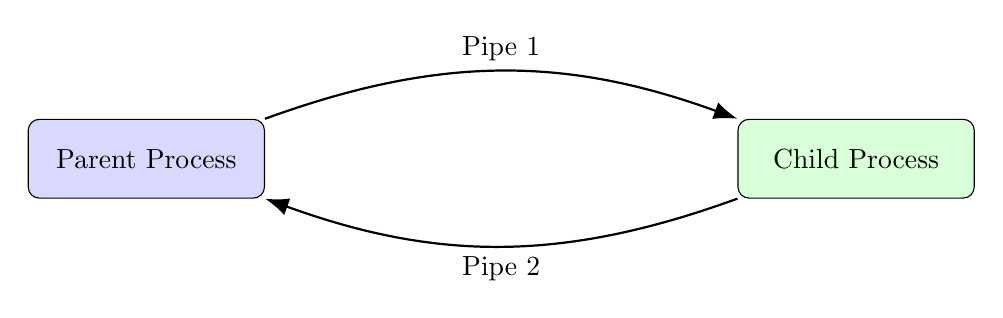
\begin{tikzpicture}[
node distance=2.5cm,
box/.style={
draw,
rounded corners,
minimum width=3cm,
minimum height=1cm,
align=center
}
]

\node[box, fill=blue!15] (parent)
{Parent Process};

\node[box, fill=green!15,
right=6cm of parent] (child)
{Child Process};

\draw[-{Latex[length=3mm]}, thick]
(parent.north east)
to[bend left=20]
node[above]{Pipe 1}
(child.north west);

\draw[-{Latex[length=3mm]}, thick]
(child.south west)
to[bend left=20]
node[below]{Pipe 2}
(parent.south east);

\end{tikzpicture}

\end{center}

\vspace{0.5cm}

This enables request-response style communication.

\end{frame}

% =====================================================
% SLIDE 31
% =====================================================
\begin{frame}[fragile]{Example: Parent Sends Number to Child}

\begin{lstlisting}[style=cstyle]
#include <stdio.h>
#include <stdlib.h>
#include <unistd.h>
#include <sys/wait.h>

int main(void)
{
    int fd[2];
    int number = 10;
    pid_t pid;

    pipe(fd);

    pid = fork();

    if (pid == 0)
    {
        int received;

        close(fd[1]);

        read(fd[0],
             &received,
             sizeof(received));

        printf("Child received = %d\n",
               received);

        close(fd[0]);
    }
\end{lstlisting}

\end{frame}

% =====================================================
% SLIDE 32
% =====================================================
\begin{frame}[fragile]{Example Continued}

\begin{lstlisting}[style=cstyle]
    else
    {
        close(fd[0]);

        write(fd[1],
              &number,
              sizeof(number));

        printf("Parent sent = %d\n",
               number);

        close(fd[1]);

        wait(NULL);
    }

    return 0;
}
\end{lstlisting}

\begin{block}{Expected Output}
\texttt{Parent sent = 10}\\
\texttt{Child received = 10}
\end{block}

\end{frame}

% =====================================================
% SLIDE 33
% =====================================================
\begin{frame}{Pipe vs FIFO}

\begin{center}
\begin{tabular}{|p{4cm}|p{4cm}|p{4cm}|}
\hline
\textbf{Feature} &
\textbf{Unnamed Pipe} &
\textbf{FIFO}
\\
\hline

Name in file system &
No &
Yes
\\
\hline

Usually used between &
Related processes &
Related or unrelated processes
\\
\hline

Creation &
\texttt{pipe()} &
\texttt{mkfifo()}
\\
\hline

Lifetime &
Normally process-related &
Can persist as filesystem object
\\
\hline

Communication &
Byte stream &
Byte stream
\\
\hline

\end{tabular}
\end{center}

\end{frame}

% =====================================================
% SLIDE 34
% =====================================================
\begin{frame}{Pipe vs Shared Memory}

\begin{center}
\begin{tabular}{|p{3.5cm}|p{4cm}|p{4cm}|}
\hline
\textbf{Feature} &
\textbf{Pipe} &
\textbf{Shared Memory}
\\
\hline

Data transfer &
Through kernel pipe buffer &
Common memory segment
\\
\hline

Programming &
Relatively simple &
More complex
\\
\hline

Synchronization &
Implicit blocking possible &
Usually explicit synchronization needed
\\
\hline

Performance &
Good for small streams &
Very fast for large shared data
\\
\hline

Typical use &
Stream communication &
High-speed data sharing
\\
\hline

\end{tabular}
\end{center}

\end{frame}

% =====================================================
% SLIDE 35
% =====================================================
\begin{frame}{Real-World Example: Shell Pipeline}

Consider:

\begin{center}
\Large
\texttt{ls | wc}
\end{center}

The shell connects:

\[
\texttt{ls}
\rightarrow
Pipe
\rightarrow
\texttt{wc}
\]

\begin{itemize}
    \item Standard output of \texttt{ls} becomes pipe input.
    \item Standard input of \texttt{wc} comes from the pipe.
\end{itemize}

This is one of the most common practical uses of pipes in Unix/Linux.

\end{frame}

% =====================================================
% SLIDE 36
% =====================================================
\begin{frame}{Standard File Descriptors}

Unix/Linux conventionally uses:

\begin{center}
\begin{tabular}{|c|c|c|}
\hline
\textbf{Descriptor} &
\textbf{Name} &
\textbf{Purpose}
\\
\hline

0 &
STDIN &
Standard Input
\\
\hline

1 &
STDOUT &
Standard Output
\\
\hline

2 &
STDERR &
Standard Error
\\
\hline

\end{tabular}
\end{center}

\vspace{0.4cm}

Using \texttt{dup2()}, a pipe can replace standard input or output.

\end{frame}

% =====================================================
% SLIDE 37
% =====================================================
\begin{frame}{What Does \texttt{dup2()} Do?}

\begin{block}{Prototype}
\centering
\texttt{int dup2(int oldfd, int newfd);}
\end{block}

Example:

\begin{center}
\texttt{dup2(fd[1], STDOUT\_FILENO);}
\end{center}

means:

\begin{center}
Send standard output into the pipe.
\end{center}

Similarly:

\begin{center}
\texttt{dup2(fd[0], STDIN\_FILENO);}
\end{center}

means:

\begin{center}
Take standard input from the pipe.
\end{center}

\end{frame}

% =====================================================
% SLIDE 38
% =====================================================
\begin{frame}{Typical Shell Pipeline Implementation}

To implement:

\begin{center}
\texttt{ls | wc}
\end{center}

we need:

\begin{enumerate}

    \item Create a pipe.
    \item Create the first child.
    \item Redirect its standard output to the pipe.
    \item Execute \texttt{ls}.
    \item Create the second child.
    \item Redirect its standard input from the pipe.
    \item Execute \texttt{wc}.
    \item Parent closes pipe descriptors and waits.
\end{enumerate}

\end{frame}

% =====================================================
% SLIDE 39
% =====================================================
\begin{frame}[fragile]{Implementation of \texttt{ls | wc}}

\begin{lstlisting}[style=cstyle]
#include <stdio.h>
#include <stdlib.h>
#include <unistd.h>
#include <sys/wait.h>

int main(void)
{
    int fd[2];
    pid_t p1, p2;

    pipe(fd);

    p1 = fork();

    if (p1 == 0)
    {
        dup2(fd[1], STDOUT_FILENO);

        close(fd[0]);
        close(fd[1]);

        execlp("ls", "ls", NULL);

        _exit(1);
    }
\end{lstlisting}

\end{frame}

% =====================================================
% SLIDE 40
% =====================================================
\begin{frame}[fragile]{Implementation Continued}

\begin{lstlisting}[style=cstyle]
    p2 = fork();

    if (p2 == 0)
    {
        dup2(fd[0], STDIN_FILENO);

        close(fd[0]);
        close(fd[1]);

        execlp("wc", "wc", NULL);

        _exit(1);
    }

    close(fd[0]);
    close(fd[1]);

    waitpid(p1, NULL, 0);
    waitpid(p2, NULL, 0);

    return 0;
}
\end{lstlisting}

\end{frame}

% =====================================================
% SLIDE 41
% =====================================================
\begin{frame}{Common Programming Mistakes}

\begin{enumerate}

    \item Using \texttt{fd[0]} for writing.

    \item Using \texttt{fd[1]} for reading.

    \item Creating the pipe after \texttt{fork()} when the processes need the
    same pipe.

    \item Forgetting to close unused ends.

    \item Ignoring return values of:
    \begin{itemize}
        \item \texttt{pipe()}
        \item \texttt{fork()}
        \item \texttt{read()}
        \item \texttt{write()}
    \end{itemize}

    \item Assuming one \texttt{read()} always corresponds exactly to one
    \texttt{write()}.

\end{enumerate}

\end{frame}

% =====================================================
% SLIDE 42
% =====================================================
\begin{frame}{Lab Execution Steps}

\begin{enumerate}

    \item Open Ubuntu/Linux terminal.

    \item Create source file:
    \begin{center}
    \texttt{nano pipe.c}
    \end{center}

    \item Compile:
    \begin{center}
    \texttt{gcc -Wall -Wextra pipe.c -o pipe}
    \end{center}

    \item Execute:
    \begin{center}
    \texttt{./pipe}
    \end{center}

    \item Verify whether the child writes successfully.

    \item Verify whether the parent receives the same data.

    \item Modify the direction of communication.

\end{enumerate}

\end{frame}

% =====================================================
% SLIDE 43
% =====================================================
\begin{frame}{Classwork}

\begin{enumerate}

    \item Create a pipe where the child sends
    \texttt{"Operating Systems Lab"} to the parent.

    \item Parent sends an integer to the child.
    The child displays the received integer.

    \item Parent sends two integers to the child.
    Child calculates and prints their sum.

    \item Child sends its PID to the parent through a pipe.

    \item Parent sends a number to the child.
    Child calculates its square and displays the result.

\end{enumerate}

\end{frame}

% =====================================================
% SLIDE 44
% =====================================================
\begin{frame}{Homework}

\begin{enumerate}

    \item Parent sends an array of integers to the child through a pipe.
    Child calculates the sum of the array.

    \item Child sends a string to the parent.
    Parent counts the number of characters.

    \item Implement bidirectional communication using two pipes.

    \item Parent sends an integer to child.
    Child computes its factorial and sends the result back to the parent.

    \item Implement the Linux command:
    \begin{center}
    \texttt{ls | wc}
    \end{center}
    using \texttt{pipe()}, \texttt{fork()}, \texttt{dup2()} and
    \texttt{exec()}.

\end{enumerate}

\end{frame}

% =====================================================
% SLIDE 45
% =====================================================
\begin{frame}{Think Before Running}

Consider:

\begin{center}
\texttt{int fd[2];}\\
\texttt{pipe(fd);}\\
\texttt{fork();}
\end{center}

Answer:

\begin{enumerate}
    \item How many processes exist?
    \item How many file descriptors does each process inherit?
    \item Which descriptor is used for reading?
    \item Which descriptor is used for writing?
    \item What happens if the reader calls \texttt{read()} before the writer
    writes?
\end{enumerate}

\end{frame}

% =====================================================
% SLIDE 46
% =====================================================
\begin{frame}{Viva Questions}

\small

\begin{enumerate}

    \item What is Inter-Process Communication?

    \item What is a pipe?

    \item Is an unnamed pipe normally unidirectional or bidirectional?

    \item What is the prototype of \texttt{pipe()}?

    \item What is the purpose of \texttt{fd[0]}?

    \item What is the purpose of \texttt{fd[1]}?

    \item Why should a pipe normally be created before \texttt{fork()}?

    \item What happens to pipe descriptors after \texttt{fork()}?

    \item What does \texttt{read()} return?

    \item What does \texttt{write()} return?

    \item Why should unused ends of a pipe be closed?

    \item What does \texttt{read()} return at end-of-file?

    \item What is \texttt{SIGPIPE}?

    \item How can bidirectional communication be implemented?

    \item Differentiate between pipe and FIFO.

\end{enumerate}

\end{frame}

% =====================================================
% SLIDE 47
% =====================================================
\begin{frame}{Session Summary}

\begin{itemize}

    \item A pipe provides Inter-Process Communication.

    \item \texttt{pipe(fd)} creates two descriptors.

    \item \texttt{fd[0]} is the read end.

    \item \texttt{fd[1]} is the write end.

    \item A pipe created before \texttt{fork()} is inherited by the child.

    \item \texttt{read()} and \texttt{write()} transfer data through the pipe.

    \item Unused pipe ends should always be closed.

    \item Traditional unnamed pipes are typically used for one-way communication.

    \item Two pipes can provide two-way communication.

    \item Unix shell pipelines are a major practical application.

\end{itemize}

\vspace{0.3cm}

\begin{center}
\Large
\textbf{Week 5 Lab Completed}
\end{center}

\end{frame}

% =====================================================
% SLIDE 48
% =====================================================
\begin{frame}{References}

\small

\begin{thebibliography}{9}

\bibitem{osc}
Abraham Silberschatz, Peter B. Galvin and Greg Gagne,
\newblock \emph{Operating System Concepts},
\newblock Wiley.

\bibitem{apue}
W. Richard Stevens and Stephen A. Rago,
\newblock \emph{Advanced Programming in the UNIX Environment},
\newblock Addison-Wesley.

\bibitem{tlpi}
Michael Kerrisk,
\newblock \emph{The Linux Programming Interface},
\newblock No Starch Press.

\bibitem{mos}
Andrew S. Tanenbaum and Herbert Bos,
\newblock \emph{Modern Operating Systems},
\newblock Pearson.

\bibitem{linuxman}
Linux Programmer's Manual,
\newblock \texttt{pipe(2)}, \texttt{read(2)},
\texttt{write(2)}, \texttt{close(2)},
\texttt{dup2(2)}.

\end{thebibliography}

\end{frame}

% =====================================================
% END
% =====================================================
\end{document}